\documentclass[a4paper, 14pt]{article}
\usepackage[pdftex,
    pdfauthor={Егоров Геннадий Викторович},
    pdftitle={Сбоник лекций по курсу радиационнной физики для 4 курса Медицинской физики},
    pdfsubject={Радиационная физика},
    pdfkeywords={ ИИ, Дозиметрия, Радиоактивность, 4 курс Медицинская физика},
    pdfproducer={LuaLatex with hyperref},
    pdfcreator={Lualatex},
    hidelinks
]{hyperref}
\usepackage{latexsym,amsmath,amssymb,amsbsy,graphicx}
\usepackage{icomma}
\usepackage{mhchem} % the canonical chemistry package(example: \ce{^{32}_{15}P})
\usepackage{multirow}
\usepackage{hhline} %Чёрточки в таблицах
\usepackage{array}
\newcolumntype{C}[1]{>{\centering\arraybackslash}p{#1}}
\graphicspath{{images/}}
\DeclareGraphicsExtensions{.pdf,.png,.jpg}
%%%%%% Для красивого отображения рисунков из inkscape
% \usepackage{import}
% \usepackage{xifthen}
% \usepackage{pdfpages}
% \usepackage{transparent}
% \newcommand{\incfig}[1]{%
%     \def\svgwidth{\columnwidth}
%     \import{./images/}{#1.pdf_tex}
% }
%%%%%%%%%%%%
\usepackage[dvipsnames]{xcolor} % dvipsnames добавляет 68 цветов https://ru.overleaf.com/learn/latex/Using_colours_in_LaTeX
\renewcommand{\emph}[1]{{\color{RedOrange}{\textit{\textbf{#1}}}}}
%%%%%%%%%%%%%%%%%%%%%%%%Оформление по ГОСТу
\usepackage{fontspec}
\setmainfont[Renderer=Basic,Ligatures={TeX}]{Times New Roman}
\usepackage[english, russian]{babel} %Поддержка русского языка
\usepackage[14pt]{extsizes} % для того чтобы задать нестандартный 14-ый размер шрифта
\usepackage{indentfirst} %Задаёт отступ самого первого абзаца
\setlength\parindent{1.25cm}
\usepackage[a4paper, left=3cm, top=1.5cm, right=1.5cm, bottom=2cm]{geometry}
\usepackage{setspace}
% \sloppy %Выравнивание текст по ширине
\onehalfspacing %Полуторный интервал
\title{Лекции по радиационной физике}
\author{Егоров Г.В. \and Пилипенко К.С.}
\date{\selectlanguage{russian}\today}
\begin{document}
\maketitle
\tableofcontents
\section{Предмет и метод радиационной биофизики. Актуальность исследования
биологического действия ионизирующего излучения. Разделы радиобиологии}
\emph{Радиационная биофизика}~---~это наука, изучающая молекулярные механизмы
биологического действия ионизирующего и неионизирующего излучения на органы,
вычисляющие последовательную картину изменений, начиная от поглощенной
энергии радиации отдельных молекул до сложных биологических изменений в клетке
и органе.

Радиационная биофизика изучает радиобиологические проблемы с позиции
биофизики. Если радиобиология изучает влияние излучения на биологические
объекты, то биофизика изучает молекулярные взаимодействия, лежащие в основе
нормальных и патологических жизненных явлений.

\emph{Ионизирующим излучением} (проникающей радиацией, ИИ) называют
высокочастотные электромагнитные излучения энергетических фотонов, которые
превышает величину потенциала ионизации больше, чем 10 эВ. К ИИ относятся рентгеновское излучение и гамма-излучение.

\noindent 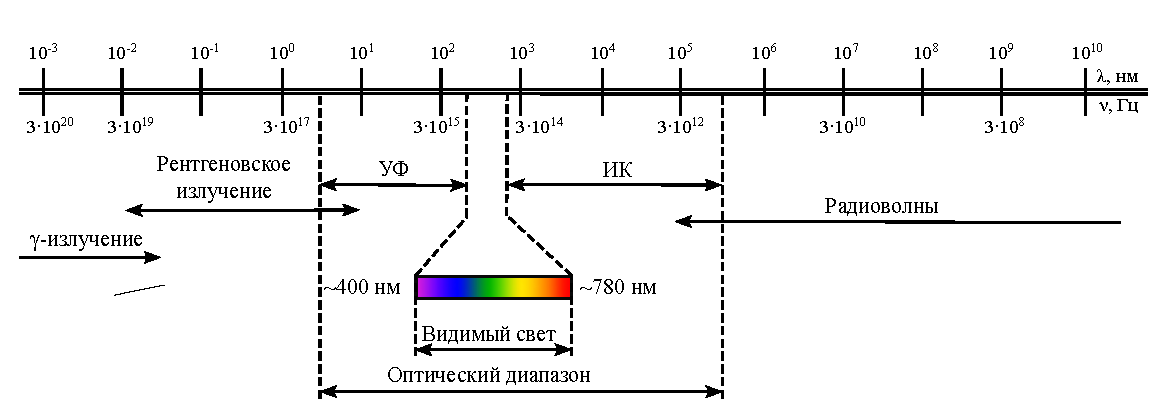
\includegraphics[width=\textwidth]{EMW.pdf}

\[ E = h\nu = \frac{hc}{\gamma}, 1\;\text{эВ} = 1,6 \cdot 10^{-19}\;\text{Дж}\]
\[ E = 10\;\text{эВ} = 1,6 \cdot 10^{-18}\;\text{Дж}\]
\[ \gamma = \frac{hc}{E} = \frac{6,6\cdot 10^{-34} \cdot 3 \cdot 10^8}{1,6 \cdot 10^{-19}} = 1,2 \cdot 10^{-7}\;\text{м} = 120\;\text{нм}\]
Рентгеновское излучение и гамма-излучение отличаются по энергии, длине
волны и по происхождению.

Рентгеновское излучение делится на \textit{тормозное} и \textit{характеристическое}.

\emph{Тормозное} возникает при торможении заряженных частиц при большом
ускорении. Энергетический спектр является непрерывным.

\emph{Характеристическое} возникает при переходах между далеко расположенными
энергетическими уровнями. Спектр излучения дискретный.

Гамма-излучение возникает либо при ядерных реакциях, либо при переходах в
энергетических уровнях в ядрах.

\emph{Оптические излучения} не способны к ионизации молекул, лишены высокой
проникающей способности.
К ИИ также относятся: корпускулярные излучения, а именно: $\beta$-частицы, т.е. электроны, позитроны, протоны, $\alpha$-частицы, так же нейтроны и др. частицы.

Актуальность исследования биологического действия ИИ:
\begin{enumerate}
    \item Все живое постоянно подвергается воздействию постоянного естественного
    радиационного фона;
    \begin{itemize}
        \item космическая радиация;
        \item излучение радиоактивных элементов, залегающих в поверхностных слоях
        земной коры и входящих в состав живых организмов и продуктов питания;
    \end{itemize}
    \item В связи с техногенной деятельностью человека (взрывы, аварии)
    радиационный фон во многих регионах значительно выше естественного, поэтому
    возникает необходимость исследования влияния этого повышенного фона на здоровье
    и жизнь человека;
    \item  ИИ используется как диагностическое и
    терапевтическое средство при многочисленных заболеваниях
\end{enumerate}
Радиационная терапия основана на изучении механизмов взаимодействия
излучения с веществом.

\emph{Радиобиология}~--~это комплексная наука, в которой развиваются многие
направления:
\begin{enumerate}
    \item Радиационная экология и генетика
    \item Радиационная биохимия и цитология
    \item Радиационная медицина и генетика
    \item Радиационная биофизика
\end{enumerate}

\emph{Радиационная биофизика} занимает особое место в радиобиологии. Она
выясняет физико-химические и молекулярные механизмы первичных процессов
лучевых изменений, протекающих с момента возникновения ионизирующего
возбуждения атомов и молекул до появления видимых структурных и функциональных изменений.

Для решения этой задачи необходимо углубленный анализ процессов,
проходимых после поглощения энергии квантов в живой системе, описание всех
этапов в терминах молекулярных изменений и создание единой картины, отражающей
всю последовательность реакций, приводящих в зависимости величины дозы к
лучевым изменениям или поражениям.

\section{История развития радиационной биофизики}
Радиобиология возникла после открытия рентгеновского излучения, которое
произошло в конце 19 веке.

В декабре 1895г., Рентгеном был сделан первый рентгеновский снимок кисти своей руки. Результаты работы были изложены в рукописи об открытии катодных проникающих Х-лучей.

В январе 1896 г. брошюра Рентгена «Новый род лучей» вышла в свет на
нескольких языках, открытие стало достоянием мировой общественности.

Март 1996, Анри Беккерель обнаружил явление~---~самопроизвольное испускание
невидимых глазу проникающих излучений ($\alpha, \beta$ и $\gamma$), исходящих от солей урана.

Через два года Мария и Пьер Кюри выделили из урановой смолы ранее не
известные элементы, так же, подобно урану, испускающие излучения, которым они
дали название радий и полоний. Для явления, свойственного этим, а в последующем
другим подобным элементам был предложен термин \emph{радиоактивность}.

Открытие урановых, а затем и ториевых лучей послужило началом
исследований \textit{естественной (природной) радиоактивности}.

1934г. Ирен Кюри и Фридерих Жулио Кюри открыли новое явление~---~искусственную радиоактивность (при исследовании ядерной реакции $^{27}Аl(\alpha,n)^{30}P$ %TODO: Нужно уточнить реакцию
обнаружили образование нового, не встречающегося ранее в природе радионуклида~---~фосфора $^{30}Р$).

\subsection{Развитие радиобиологии}
Петербуржский физиолог Тарханов провел исследование на лягушках и
насекомых и пришел к выводу, что Х-лучами можно не только фотографировать, но и
влиять на ход жизненных функций.

Ефим Лондон в 1896 году начал исследование по экспериментальной
радиобиологии.

Первая официальная информация о патологическом влиянии радиации была
опубликована в 1901 году, которая сообщила, что радий вызывает ожоги кожи.

\emph{Важными задачами} радиобиологии в то время была необходимость точной и
количественной оценки дозы радиации, вначале появились условные единицы
биологических доз.

% HED (кожная-эритемная доза) %TODO: Зачем это здесь?
В 1901 и последующие годы появилось множество работ о лучевом поражении
кожи. В 1902 году описан первый случай лучевого рака кожи. Выяснилось, что
возникающая радиация не только воздействует на кожу, но и вызывает лучевое
поражение внутренних органов и тканей, а также гибель живых организмов и
человека. Опыты Лондона в России и Хейкеля в Германии.

В Последующие годы выяснились сведения о высокой биологической эффективности нового вида излучений стимулировало мощный взрыв радиобиологических работ, характеризующий \emph{начальный, описательный период} в истории радиобиологии.  

\subsection{Открытие закона радиочувствительности клеток}
В 1906 г. французские радиобиологи Жан Бергонье и Луи Трибондо сформулировали фундаментальный \emph{закон (правило) радиочувствительности клеток:} \textit{ ИИ оказывает тем большее повреждающее действие на клетки, чем интенсивнее те делятся и чем менее определенно выражены их морфология и функция, т. е. чем менее они дифференцированны}. 

По мере накопления фактов становилось ясным, что ИИ, в зависимости от интенсивности источника радиации и длительности облучения, способны вызывать повреждения и гибель любого биологического объекта, любой биологической системы.

Начиная с 1910 г. М. И. Неменов и сотрудники публикуют работы по
выяснению изменений обмена веществ при лучевом поражении и о сходстве лучевых
изменений с процессами патологии раннего старения.

Первая в мире монография (Е. С. Лондон <<Радий в биологии и медицине>>)
вышла в свет в 1911 г. на немецком языке, а в 1968 г. переведена на русский язык в
издательстве \textit{<<Медицина>>}.

В 1918 г. в Петербурге был открыт первый в стране радиобиологический
Государственный институт рентгенологии и радиологии, организатором
и директором стал рентгенолог М. И. Неменов.

В 1925 г. была наглядно показана важная роль биохимических процессов в
развитии лучевого поражения. Анцель и Винтенбергер в опытах на куриных
эмбрионах обнаружили, что интенсивность обменных процессов оказывается
основополагающей в формировании проявлений лучевого поражения. Это
наблюдение позволило авторам предсказать участие трех существенных моментов в
развитии лучевого поражения:
\begin{itemize}
    \item \textit{наличие первичного радиационного повреждения;}
    \item \textit{существование факторов, способствующих усилению этого повреждения;}
    \item \textit{влияние восстанавливающих факторов.}
\end{itemize}

Постепенно формировалось представление, согласно которому степень лучевого
поражения определяется не только интенсивностью первичного
повреждения, но и физиологическим состоянием организма и характером
метаболических процессов в нем. Для возникновения острой лучевой болезни
должен произойти сложный комплекс взаимосвязанных изменений в организме,
появление которых зависит от величины дозы, характера и способа облучения, от
времени, прошедшего после лучевого воздействия и биологической особенности
организма (его радиочувствительности).

Исследование динамики и механизмов формирования биохимических нарушений при лучевых поражениях заняло все дальнейшие годы развития радиобиологии и позволило собрать ценнейший материал для характеристики и классификации клинических проявлений радиационного эффекта. Это привело исследователей к установлению количественных принципов, связывающих радиобиологические эффекты с дозой облучения. 

\subsection{Появление количественной радиобиологии}
В 20-е годы XX в. был открыт следующий, \emph{второй период в развитии радиобиологии – период изучения механизмов действия ИИ на биологические объекты и системы} и положено начало формированию \emph{количественной радиобиологии}. Начались интенсивные поиски критических биологических молекулярных и клеточных структур, а также органов и тканей облучаемых организмов, ответственных за развитие лучевого поражения, ведущего к смертельному исходу.

\emph{Открытие радиобиологического парадокса:} энергия ИИ несопоставима мала по сравнению с тем эффектом, который она вызывает (в тепловом измерении). 

В 1925-1927 гг. советскими учеными Г.А.Надсоном и Г. С. Филипповым обнружили в экспериментах на дрожжевых клетках, а позднее Г. Мѐллером (США) на дрозофиле \emph{эффекта радиационного мутагенеза}, проявляющегося не только в повреждении \textit{«вещества наследственности»}, но и в образовании стойких необратимых изменений в нем, передающихся по наследству. Были получены строгие доказательства возникновения мутаций под влиянием облучения. 

С открытием мутагенного действия излучений многие радиобиологи перешли к изучению \emph{ единичной реакции дискретных биологических структур (генов, хромосом) на радиационное воздействие}. В это же время значительно совершенствуются методы дозиметрии излучений, вводится ионизационная единица дозы – рентген. 

Появляется возможность количественного анализа биологического действия излучений, основанного на выяснении зависимости между наблюдаемым биологическим эффектом и дозой радиации, поглощенной изучаемой системой. Такие эксперименты проводились не только на ядерных наследственных структурах, но и на колониях клеток, вирусных частицах, препаратах ферментов. Результаты, полученные в точных количественных опытах, свидетельствовали о вероятностном характере проявления единичной реакции объекта в ответ на облучение в данной дозе радиации. 
% Иначе говоря, при облучении однородных объектов (клетки одной линии, молекулы одного типа и т.д.) наблюдали, что при любой малой дозе радиации некоторое число объектов оказывается пораженным, а другие сохраняют исходные свойства; \emph{при самой большой дозе радиации небольшая доля объектов все еще остается непораженной. Кривые «доза-эффект» в этих случаях имели
% экспоненциальный характер} и их можно было надежно экстраполировать к нулевой
% точке.

Обнаруженный эффект нельзя было объяснить естественной вариабельностью:
речь шла о генетически однородных клетках и вирусных частицах или молекулах
одного типа. Его трактовка потребовала прежде всего, представлений о
вероятностном характере поглощения энергии излучений, о дискретной природе
частиц, составляющих  ИИ, о физически микрогетерогенной
организации биологических структур.

Начало исследований в области количественной радиобиологии (20-е гг.) и
стало рождением радиационной биофизики, так как впервые для объяснения
радиобиологических феноменов и создания общей теории биологического действия
 ИИ в качестве отправных концепций потребовалось
использовать теоретические положения квантовой механики и ядерной физики.

В 1922 г. Ф. Дессауэр, предложил \emph{теорию «точечного нагрева»}.
 ИИ обладают малой объемной плотностью, однако отдельные
фотоны несут гигантский запас энергии. Ф. Дессауэр предположил, что при
поглощении системой относительно небольшой общей энергии (смертельная для
человека доза облучения вызывает нагрев тела всего на 0,001$^\circ$С) некоторые
дискретные микрообъемы поглощают настолько большие порции энергии, что
действие  ИИ можно сравнить с таким микролокальным
нагревом, который вызывает глубокие структурные изменения и в конечном счете
биологическое поражение. Вероятностный характер проявления эффекта у
отдельных объектов автор гипотезы объяснял статистическим распределением
\textit{«точечного тепла»}. Так впервые \emph{физический принцип попадания был использован
в исследованиях количественной радиобиологии}.

Дальнейшее его развитие связано с работами Дж. Кроутера, Д. Ли, К. Г. Циммера, Н. В. Тимофеева-Ресовского, В. И. Корогодина и др. 

Работы этого периода оказали большое влияние на дальнейшее развитие радиационной биофизики, превратили ее в одну из самых точных биологических дисциплин. Математический аппарат, развитый в этих работах, позволил с достаточной надежностью судить о \textit{«пусковых событиях»}, приводящих к регистрируемым в эксперименте биологическим реакциям (мутации, гибель клетки и др.) и оценивать параметры «мишени», ответственной за наблюдаемый радиобиологический эффект.
% Согласно \emph{принципу попадания}, начальный физический пусковой механизм, необходимый для возникновения конечной биологической реакции, обусловлен случайным взаимодействием ионизирующего излучения с веществом. В силу этого в каждую молекулу или клетку происходит неодинаковое число попаданий. С принципом попаданий тесно связана \emph{теория мишени}, основанная на принципе гетерогенности строения живых систем, поражение излучением отдельных элементов которых имеет не одинаковое значение для данной системы. Например, необратимое повреждение уникальной клеточной структуры фатально для клетки, тогда как такое же повреждение иных, множественных структур для судьбы клетки может иметь существенно меньшее значение. 
В многочисленных работах получены новые факты высокой радиочувствительности делящихся клеток, клеточного ядра, молекулы ДНК. 

Сейчас хорошо известно, что \emph{высокой радиочувствительностью обладают делящиеся клетки, клеточное ядро и молекула ДНК}, причём нарушения генетических структур могут проявляться как сразу после облучения, так и отдаленно, в потомках, даже спустя несколько поколений, становясь в организме причиной возникновения злокачественных опухолей, а также различных уродств развития. 
%TODO:
% Обнаруженный эффект можно объяснить, используя представления о вероятностном характере поглощения энергии излучений и о дискретной природе частиц, составляющих  ИИ. 

Выяснилось, что даже при облучении в малых дозах происходит много тысяч актов ионизации молекул, но лишь некоторые из образовавшихся нарушений структуры и функции клеток приводят клетку к потере способности деления и гибели. 

\emph{Критической мишенью клетки является молекула ДНК.} Применение теории мишени ограничено. Конкретная ответная реакция на облучение зависит не только от попадания ДНК, но и от ряда свойств самого биологического объекта, например, от способности устранять повреждения - системный ответ клетки на облучение. 

Системный ответ носит \textit{статистический характер}. Важным направлением в статистической физике является создание математической модели, которая является формализованным выражением теоретических закономерностей. Усовершенствование моделей связано с повышением доступности и быстродействием компьютеров. 

% \subsection{Появление радиационной биофизики}
Радиационная биофизика зародилась в 20 г. ХХ в., когда впервые для объяснения радиобиологических явлений стали использовать теоретические положения квантовой механики и ядерной физики. 

Согласно \emph{принципу попадания} начальный физический пусковой механизм, необходимый для возникновения биологической реакции обусловлен случайным взаимодействием ИИ с веществом. 

С принципом попадания связана \emph{теория мишени}, основанная на принципе гетерогенности. Необратимое повреждение уникальной клеточной структуры фатально для клетки, тогда как такое же повреждение других структур имеет меньшее значение. 

В середине ХХ столетия после бомбардировок Хиросимы и Нагасаки начался \emph{3 этап в развитии радиобиологии}. Происходит перенос акцентов в развитии радиологии и радиационной биофизики. Развиваются исследования молекулярных механизмов действия излучения. Этому способствовал ряд достижений в области биофизики и молекулярной биологии, а именно доказательство биологической роли ДНК и расшифровка ее структуры. 

В 40-е гг. было обнаружено зарождение в облучаемом растворе высокоактивных продуктов \emph{радиолиза воды} – свободных радикалов, способных диффундировать на значительные расстояния и поражать биологические структуры. 

Радиационная биофизика начинает оперировать представлениями о \emph{«непрямом действии»} излучения, опосредованном активными продуктами радиолиза воды. 

Были изучены физико-химические свойства первичных продуктов радиолиза воды и характер их взаимодействия с макромолекулами клетки. Это дало возможность приступить к исследованиям средств защиты (\emph{радиопротекторов}) от действия  ИИ. 

В 1942 г. В. Дейлу удается снизить поражающее действие радиации на ферменты введением в раствор ряда веществ – перехватчиков радикалов. 

В 1949 была доказана способность ряда веществ защищать млекопитающих от лучевого поражения. В опытах Х. Патта с соавторами введение цистеина за 10 мин до облучения защищало крыс от неминуемой гибели. 

В мире начинается интенсивный поиск эффективных радиозащитных препаратов. Формируется самостоятельное направление радиационной биофизики – выяснение механизмов модифицированной радиочувствительности биологических объектов. 

Было установлено, что важную роль в радиозащитных препаратах играет понижение содержания кислорода в тканях. 

В середине 60-х гг. З. Бак и П. Александер сформулировали \emph{гипотезу «биохимического шока»}, согласно которой различные радиопротекторы однотипно изменяют метаболические процессы, переводя клетки в состояние повышенной устойчивости к действию ионизирующей радиации. 

В дальнейшем появился ряд исследований, посвященных анализу конкретных биохимических изменений, возникающих под влиянием радиозащитных агентов и модифицирующих радиорезистентность организма. Возникли гипотезы «комплексного биохимического механизма действия радиозащитных средств», «сульфгидрильная гипотеза». 

Исследования привели к накоплению обширного фактического материала по общей картине лучевого поражения и его модификации, они позволили наметить пути к выявлению основных закономерностей зарождения пусковых физико-химических процессов, механизмов ослабления или усиления первичных лучевых реакций. В результате на первый план вышли исследования, посвященные анализу физико- химических процессов, протекающих в клетке от момента возникновения начальных структурных повреждений до проявления выраженных биохимических и морфологических изменений. 

Анализируется модифицирующее действие кислорода, температуры и других агентов, влияющих на развитие лучевого поражения биологических объектов. 

Авария на Чернобыльской АЭС в 1986 г., снятие секретов с информации о ее последствиях, последствиях других радиационных аварий и ядерных испытаний открыли новый, \emph{четвертый период в истории радиобиологических исследований}.

Для решения проблем, возникших после Чернобыльской катастрофы, накопленные знания и имеющийся опыт традиционной радиобиологии н медицины оказываются явно недостаточными, и поэтому в современной радиобиологии стали быстро развиваться новые направления: 

\begin{itemize}
    \item изучение биологического действия излучений в малых дозах и отдаленных последствий облучения; 
    \item исследование комбинированного действия широкого спектра радионуклидов с химическими загрязнителями среды; 
    \item поиск принципиально новых средств защиты от хронического облучения. 
\end{itemize}

Перед радиационной биофизикой возникли новые задачи. Наиболее важными оказались фундаментальные исследования механизмов радиобиологических эффектов, вызываемых слабыми воздействиями, поскольку оказалось, что эффекты, вызываемые  ИИ в малых дозах, нельзя оценивать путем простой экстраполяции в область малых доз данных, полученных при больших дозах. 

Открылись \emph{принципиально новые явления при изучении эффектов малых доз}. Это и повышенная чувствительность биообъектов к воздействию радиации в сверхмалых дозах, переходящая к повышенной радиорезистентности – \emph{адаптивному ответу} – при более высоких нелетальных дозах. Это и \textit{стимулирующее действие излучений на рост, развитие и другие физиологические показатели} (эффект гормезиса), а также \textit{необычное снижение выраженности радиобиологических эффектов по мере увеличения мощности малой дозы} (\emph{обратный эффект мощностей доз}). 

Кривая зависимости \emph{доза-эффект} в области малых доз синусоидальная. 

Большое значение приобретают исследования механизмов регуляции, происходящих в биоматериале (БМ) и ДНК и образующихся в них под действием  ИИ оксирадикалов и других продуктов окисления. 

На рубеже столетий было открыто важное явление: \textit{способность облученной клетки передавать путем контактов или секреции сигналы, действующие на соседние необлученные клетки подобно облучению}~---~\emph{эффект свидетеля}. 

Современный период диктует новые переходы к разработке методов химической защиты. Появилась необходимость в исследованиях пищевых продуктов и препаратов, способных, не оказывая вредного побочного действия на организм снижать или предотвращать хроническое низкоинтенсивное облучение. Большое внимание уделяется средствам, выводящим радионуклиды из организма.

\section{Виды и характеристики ионизирующих излучений}
К ионизирующим излучениям относят: фотоны электромагнитного излучения ($\lambda < 20$ нм) и корпускулярное излучение, т.е. ускоренные частицы и ядра электронов.

Фотонное излучение делится на: рентгеновское (до 500 кэВ) и $\gamma$-{\nolinebreak}излучение
(более 500 кэВ).

Рентгеновское:
\begin{itemize}
    \item $E_\text{ф}<$ 50 кэВ- мягкое ($\lambda > 25$ нм);
    \item $E_\text{ф}>$ 50 кэВ- жесткое ($\lambda < 25$ нм).
\end{itemize}
От 25~нм до $2,5\cdot 10^{-3}$~нм рентгеновское излучение.
Рентгеновское излучение возникает двумя путями:
\begin{enumerate}
    \item характеристическое рентгеновское излучение – при переходах между
    далеко расположенными энергетическими уровнями;
    \item тормозное рентгеновское излучение возникает при торможении частиц
    высоких энергий (кинескоп).
\end{enumerate}
\emph{$\gamma$-излучение}~---~электромагнитное излучение, возникающее при ядерных реакциях. От
50 кэВ до 10 МэВ

Эти диапазоны энергии излучений перекрываются и отличаются по происхождению. Рентгеновское возникает: 
\begin{itemize}
    \item при переходах между далеко расположенными уровнями в атоме (характеристическое рентгеновское излучение);
    \item либо при торможении быстрых частиц (тормозное излучение). 
\end{itemize}

В свою очередь $\gamma$-излучение возникает: 
\begin{itemize}
    \item при переходах при различных ядерных превращениях;
    \item либо при переходах в ядрах.
\end{itemize} 

\emph{К корпускулярному излучению} относят электроны, позитроны, нейтроны, $\alpha$-частицы, протоны, ускоренные ионы, ядерные фрагменты и осколки деления ядер, а также многие нестабильные частицы. 

\emph{К электронному излучению относят} $\beta$-частицы (электроны с энергией 0,002~--~2,3 МэВ, возникающие при распаде радиоактивных ядер) и ускоренные электроны, которые создаются ускорителями электронов (с энергией от кэВ до сотен МэВ). 

Ядра атома гелия называются $\alpha$-частицами, когда они образуются при распаде некоторых радионуклидов и несут энергию до $\sim$10 МэВ. Те же ядра, ионизированные и ускоренные, образуют пучки ионов гелия. Эти и другие пучки заряженных частиц – протонов, дейтронов и вообще любых многозарядных тяжелых ионов (например, углерода) – получают в протонных и ионных ускорителях. На них при облучении мишеней получают также пучки нейтральных частиц – фотонов и нейтронов, и даже пучки радиоактивных ионов. 

Наиболее интенсивные потоки нейтронов получают при делении ядер урана и плутония в ядерном реакторе, а также в нейтронных генераторах. Нейтронное деление имеет широкий спектр энергий с максимумом при 1~--~2~МэВ.

\subsection{Линейная передача энергии излучения}
Путь частицы в веществе можно наблюдать по произведенному ей эффекту.
\textit{Ионизирующий след} заряженной частицы называют \textit{треком}. Действие ионизирующего
излучения на вещество характеризуется с помощью \emph{ЛПЭ~---~линейной передачи
энергии}.

ЛПЭ~---~величина, равная средней потере энергии частицы на единицу пути
первичной заряженной частицы в пределах объема ее трека; измеряется в кэВ/мкм.

Обычно принимается, что вещество – это вода с плотностью 1 г/см$^3$, и поэтому
ЛПЭ измеряется в единицах кэВ/мкм. Таким образом, вводится различие между ЛПЭ
и удельными ионизационными потерями энергии частицы, в которых учитывается не
только выделенная локально, но и вся энергия, потерянная при прохождении частицей
1 г/см$^2$ вещества.

Характерной величиной является 0,2 кэВ/мкм (к этой минимальной величине
довольно близки ЛПЭ в очень широком диапазоне –для электронов всех энергий и
фотонов выше 0.5 МэВ).

Еще одно различие: по мере прохождения частиц вглубь среды их энергия
изменяется как бы непрерывно, то есть часто теряется малыми порциями за счет
ионизации атомов среды. Иначе происходит изменение энергии фотонов и нейтронов
– это более редкие события, обычно с большой передачей энергии сразу, без
образования треков, и проследить, как меняется энергия частицы, становится трудно.
Поэтому к ним вообще не применяется понятие ионизационных потерь энергии, а
говорить об ЛПЭ фотонов или нейтронов можно всегда, это практически удобно. В
этом и заключается причина, почему радиационная физика перешла на «язык ЛПЭ»
(линейных передач энергии).

Когда говорят просто об удельных потерях энергии частицы ($–dE/dx$; знак минус
часто не ставится), то обычно подразумевают «ионизационные потери».

При делении линейных потерь энергии на плотность вещества р получаем
значение $(–dE/dx)/p$, которое не зависит от плотности. Эту величину тоже можно
называть тормозной способностью вещества, или даже ЛПЭ, и тогда она измеряется в
МэВ/см$^2\cdot$г$^{-1}$.

Зная ЛПЭ, легко определить среднее число ионов, образованных на единицу
пути частицы. Для этого достаточно разделить значение ЛПЭ на величину энергии,
необходимой для образования одной пары ионов (W). Отношение $L/W$ называют
\emph{линейной плотностью ионизации} (ЛПИ).

Точное значение \emph{W} тканей определить трудно. Для газов значение \emph{W} было
измерено многими исследователями, оно составляет около 34 эВ.
$\text{ЛПИ} = \frac{\text{ЛПЭ}}{W}$, W~---~энергия, необходимая для образования одной пары ионов
(W=34эВ).

Для оценки \emph{плотности ионизации}: $\text{ЛПИ} = \frac{\text{ЛПЭ}}{34}$.

Чем выше ЛПЭ, тем больше теряет энергии частица на единицу пути, тем
плотнее распределены ионы вдоль трека.

\section{Радиоактивность. Изотопы. Закон радиоактивного распада. Типы
радиоактивного распада ($\alpha$- и $\beta$-распад)}

\emph{Радиоактивность}~---~явление, которое заключается в самопроизвольном
превращении (распаде) атомных ядер некоторых химических элементов в атомные
ядра других элементов с испусканием особого рода излучения.
\emph{$\alpha$-ядра гелия, $\beta$-поток электронов}.

\ce{^{A}_{Z}X} \rightarrow \ce{^{A-4}_{Z-2}Y} + \ce{^{4}_{2}He}~---~$\alpha$-распад

\ce{^{A}_{Z}X} \rightarrow \ce{^{A}_{Z+1}Y} + \ce{^{0}_{-1}e} + \ce{^{0}_{0}$\tilde{\nu}$ }~---~$\beta$-распад

\ce{^{A}_{Z}X} \rightarrow \ce{^{A}_{Z-1}Y} + \ce{^{0}_{+1}e} + \ce{^{0}_{0}$\tilde{\nu}$ }~---~позитронный $\beta$-распад

\ce{^{1}_{0}n} \rightarrow \ce{^{1}_{1}p} + \ce{^{0}_{-1}e} + \ce{^{0}_{0}$\tilde{\nu}$ }

\ce{^{1}_{1}p} \rightarrow \ce{^{1}_{0}n} + \ce{^{0}_{+1}e} + \ce{^{0}_{0}$\tilde{\nu}$ }

Реакция электронного $\beta$-распада проходит естественным путем, в отличии от
позитронного $\beta$-распада.

У многих электронов ядра могут иметь несколько разновидностей,
отличающихся числом нейтронов в ядре и их называют \emph{изотопами} (\ce{^{12}_{6}C}, \ce{^{14}_{6}C}; \ce{^{1}_{1}H}, \ce{^{2}_{1}H}~---~дейтерий, \ce{^{3}_{1}H}~---~тритий).

\subsection{Закон радиоактивного распада}
Закон радиоактивного распада описывает зависимость интенсивности радиоактивного распада от времени и от количества радиоактивных атомов в образце. В дифференциальной форме уравнение имеет следующий вид: 
\begin{equation}
    \frac{dN}{dt} = - \lambda t
\end{equation}
В интегральной формулировке принимает вид:
\begin{equation}
    N = N_0 \cdot e^{-\lambda t} = N_0 \cdot 2^{-\frac{t}{T}},
\end{equation}
где  $\lambda$~---~постоянная распада, T~---~период полураспада ($\lambda = \frac{ln2}{T}$), N число нераспавшихся ядер спустя время t.

\subsection{Активность радиоактивного элемента}
Количество радиоактивного вещества определяется не только массой, но и
активностью.

\emph{Активность (А)}~---~\textit{это мера радиоактивности какого-либо количества
радионуклида, равная среднему числу распадов в единицу времени.}
\begin{equation}
    A = \frac{dN}{dt},
\end{equation}
где $dN$~---~ожидаемое число спонтанных ядерных превращений из
данного энергетического состояния за промежуток времени $dt$.

\emph{В СИ:} [А] = 1~Бк (Беккерель)

1 Бк $ \rightarrow $ 1 распад за 1~с

Внесистемная единицы: 1 Кюри~---~это активность 1 г радия.

1 Кю = $3,7 \cdot 10^{10}$~Бк, 1 Бк = $2,7\cdot 10^{-11}$~Ки

Концентрация активности радиоактивного вещества часто определяется
величиной удельной $А_m$ (или объемной $А_v$) активности, представляющей отношение
активности (А) радионуклида в исследуемом веществе к его массе (т) или объему (V).

\section{Дозиметрия}
\emph{Дозиметрия}~---~раздел физики, изучающий воздействие ионизирующих
излучений на объекты живой и неживой природы, а также методы измерения действия
излучения.
\begin{table}[htbp]
    \centering\begin{tabular}{|*{4}{C{1.6cm}|}|*{4}{C{1.6cm}|}}
        \hhline{|-|-|-|-||-|-|-|-|}
        \multirow{2}{1.6cm}{Множитель} & \multirow{2}{1.6cm}{Приставка} & \multicolumn{2}{c||}{Обозначение} & \multirow{2}{1.6cm}{Множитель} & \multirow{2}{1.6cm}{Приставка} & \multicolumn{2}{c|}{Обозначение} \\ \hhline{|~|~|-|-||~|~|-|-|}
        & & русское & международное & & & русское & международное \\ \hhline{|-|-|-|-||-|-|-|-|}
        $10^{18}$ & экса & Э & E & $10^{-1}$ & деци & д & d \\ \hhline{|-|-|-|-||-|-|-|-|}
        $10^{15}$ & пета & П & P & $10^{-2}$ & санти & с & с \\ \hhline{|-|-|-|-||-|-|-|-|}
        $10^{12}$ & тера & Т & T & $10^{-3}$ & милли & м & m \\ \hhline{|-|-|-|-||-|-|-|-|}
        $10^{9}$ & гига & Г & G & $10^{-6}$ & микро & мк & $\mu$ \\ \hhline{|-|-|-|-||-|-|-|-|}
        $10^{6}$ & мега & М & M & $10^{-9}$ & нано & н & n \\ \hhline{|-|-|-|-||-|-|-|-|}
        $10^{3}$ & кило & к & k & $10^{-12}$ & пико & п & p \\ \hhline{|-|-|-|-||-|-|-|-|}
        $10^{2}$ & гекто & г & h & $10^{-15}$ & фемто & ф & f \\ \hhline{|-|-|-|-||-|-|-|-|}
        $10^{1}$ & дека & да & da & $10^{-18}$ & атто & а & a \\ \hhline{|-|-|-|-||-|-|-|-|}
    \end{tabular}
    \caption{Таблица приставок для образования десятичных кратных и дольных единиц}
    \label{<label>}
\end{table}

\subsection{Поглощённая доза}
Для оценки действия облучения на живые системы используют понятие
поглощенной дозы \emph{D}.

\emph{D}~---~это величина энергии ионизирующего излучения, переданная веществу, которая определяется формулой:
\begin{equation}
    D = \frac{d\left\langle E \right\rangle }{dm},
\end{equation}
где \emph{d$\left\langle E \right\rangle$}~---~средняя энергия, переданная ионизирующим излучением веществу, находящемуся в элементарном объеме, a \emph{dm}~---~масса вещества в этом объеме.

На пучке заряженных частиц (электроны, протоны и др.) поглощенная доза
рассчитывается из следующего соотношения: $D = 1,602\cdot 10^{-10}\cdot \left\langle L \right\rangle\text{Ф}$, где \emph{L}~---~средняя ЛПЭ
в единицах МэВ$\cdot \text{г}^{-1}\text{см}^2$, \emph{Ф}~---~флюенс частиц, то есть отношение dN/dS, если dN~---~количество частиц, падающих на площадку \emph{dS} см$^2$. Множитель $1,602\cdot 10^{-10}$ численно равен заряду электрона.

\textit{Энергия может быть усреднена по любому определенному объему, и в этом
случае средняя доза будет равна полной энергии, переданной объему, деленной на
массу этого объема.}

В \emph{СИ}: $[D] = \frac{\text{Дж}}{\text{кг}}$ = Грей, 1~Гр = 1~$\frac{\text{Дж}}{\text{кг}}$

Один Грей~---~это поглощенная доза ионизирующего излучения любого вида, при
которой в 1 кг массы вещества поглощается 1 Дж энергии излучения.

Используется так же и понятие мощности поглощенной дозы: [1 Гр⁄с].

Существует внесистемная единица: 1 рад = $10^{-2}$~Гр, 1 Гр = 100 рад.

\subsection{Экспозиционная доза излучения}
% Размерность экспозиционной дозы – это заряд, возникающий в единице массы поглотителя.
\emph{Экспозиционная доза (X)}~---~\textit{это количественная характеристика ионизирующей
способности рентгеновского или $\gamma$-излучения в воздухе 
% (в диапазоне энергий излученияот десятков кэВ до 3 МэВ)
, измеренная по количеству образованных зарядов (пар
ионов) в воздухе}. Экспозиционная доза определяется по формуле:
\begin{equation}
    X = \frac{dq}{dm},
\end{equation}
где $dq$~---~полный заряд ионов одного знака,
возникающих в сухом воздухе при торможении всех вторичных электронов,
образованных фотонами в малом объеме воздуха; $dm$~---~масса воздуха в этом объеме.

В \emph{СИ:} $[X] = \frac{\text{Кл}}{\text{кг}}$ (в кулонах на килограмм воздуха). На практике применяется внесистемная единица: \emph{1 Рентген}.

1 Р = $2,58\cdot 10^{-4}$~Кл/кг, 1 Кл/кг = 3876 Р

Для характеристики распределения во времени экспозиционной дозы
используют величину \emph{мощности дозы ($\frac{X}{t}$)}. 1 Р/с = $2,58\cdot 10^{-4}$~Кл/(кг$\cdot$с), 1 Кл/(кг$\cdot$с) = 3876 Р/с

Общая формула, связывающая величину экспозиционной дозы излучения X с
активностью препарата А:
\begin{equation}
    X = \frac{AtK_\gamma}{R^2},
\end{equation}
где \emph{активность А} выражается в мКюри, \emph{t}~---~время облучения в часах; \emph{$K_\gamma$}~---~\mbox{$\gamma$}-постоянная данного изотопа в Р/ч; расстояние от
источника излучения до измеряемого объекта \emph{R} в см. При этом доза излучения будет
выражена в рентгенах.

\subsection{Эффективная доза облучения}
Еще одним типом взвешивающих коэффициентов $W_T$ для оценки радиочувствительности биологических систем является \emph{эффективная доза облучения}~---~\textit{это величина, используемая как мера возникновения риска отдаленных последствий облучения всего тела человека и отдельных его органов и тканей с учетом радиочувствительности.} 

Она представляет сумму произведений эквивалентной дозы в органах и тканях на соответствующие взвешивающие коэффициенты: 
\begin{equation}
    E = \sum W_T \cdot H_T,
\end{equation} 
где $H_T$~---~эквивалентная доза в органе или ткани Т, $W_T$~---~взвешивающий коэффициент для органа или ткани Т. 
Эффективные дозы измеряются так же, как и эквивалентные, в бэрах и зивертах.
\begin{table}[htbp]
    \centering\begin{tabular}{|p{12cm}|C{3,5cm}|}
        \hline
        \emph{Орган или ткань} & \emph{Значение  коэффициента} $W_T$ \\ \hline
        Гонады & 0,20 \\ \hline
        Костный мозг (красный) & 0,12 \\ \hline
        Толстый кишечник (прямая, сигмовидная, нисходящая) & 0,12 \\ \hline
        Легкие & 0,12 \\ \hline
        Желудок & 0,12 \\ \hline
        Мочевой пузырь & 0,05 \\ \hline
        Грудная железа & 0,05 \\ \hline
        Печень & 0,05 \\ \hline
        Пищевод & 0,05 \\ \hline
        Щитовидная железа & 0,05 \\ \hline
        Кожа & 0,01 \\ \hline
        Клетки костных поверхностей & 0,01 \\ \hline
        Остальные & 0,05 \\ \hline
        \emph{Сумма всех $W_T$} & \emph{1,00} \\ \hline
    \end{tabular}
    \caption{Радиочувствительность отдельных органов и тканей}
    \label{<label>}
\end{table}

\end{document}